\documentclass[11pt]{article}

\usepackage{titling}
\renewcommand\maketitlehooka{\null\mbox{}\vspace*{0.20\textheight}}
\renewcommand\maketitlehookd{\vfill\null}

\usepackage{graphicx}
\usepackage[margin=1.0in]{geometry}
\usepackage{hyperref}
\usepackage{courier}
\usepackage{color}
\definecolor{mygreen}{rgb}{0,0.6,0}
\definecolor{mygray}{rgb}{0.5,0.5,0.5}
\definecolor{mymauve}{rgb}{0.58,0,0.82}

\usepackage{listings}

\lstset{ 
  backgroundcolor=\color{white},   % choose the background color; you must add \usepackage{color} or \usepackage{xcolor}; should come as last argument
  basicstyle=\footnotesize\ttfamily,        % the size of the fonts that are used for the code
  breakatwhitespace=false,         % sets if automatic breaks should only happen at whitespace
  breaklines=true,                 % sets automatic line breaking
  captionpos=b,                    % sets the caption-position to bottom
  commentstyle=\color{mygreen},    % comment style
  deletekeywords={...},            % if you want to delete keywords from the given language
  escapeinside={\%*}{*)},          % if you want to add LaTeX within your code
  extendedchars=true,              % lets you use non-ASCII characters; for 8-bits encodings only, does not work with UTF-8
  keepspaces=true,                 % keeps spaces in text, useful for keeping indentation of code (possibly needs columns=flexible)
  keywordstyle=\color{blue},       % keyword style
  language=C++,                    % the language of the code
  morekeywords={*,...},            % if you want to add more keywords to the set
  numbers=left,                    % where to put the line-numbers; possible values are (none, left, right)
  numbersep=10pt,                   % how far the line-numbers are from the code
  numberstyle=\tiny\color{mygray}, % the style that is used for the line-numbers
  rulecolor=\color{black},         % if not set, the frame-color may be changed on line-breaks within not-black text (e.g. comments (green here))
  showspaces=false,                % show spaces everywhere adding particular underscores; it overrides 'showstringspaces'
  showstringspaces=false,          % underline spaces within strings only
  showtabs=false,                  % show tabs within strings adding particular underscores
  stepnumber=1,                    % the step between two line-numbers. If it's 1, each line will be numbered
  stringstyle=\color{mymauve},     % string literal style
  tabsize=2,	                   % sets default tabsize to 2 spaces
  title=\lstname                   % show the filename of files included with \lstinputlisting; also try caption instead of title
}


\title{C++ AutoGarbage\\\medskip
\large An automatic mark and sweep garbage collector for the C++ Programming Language}
\author{Michael Lynch}
\date{\today}
\hypersetup{
pdfauthor={Michael Lynch},
pdftitle={C++ AutoGarbage},
pdfsubject={Garbage Collection},
pdflang={English}}
\begin{document}
\begin{titlingpage}
\maketitle
\end{titlingpage}
\newpage

\vspace*{0.15\textheight}
\emph{Abstract.} C++ has become one of the most popular languages in the world, partially through its capability for
very deep control over memory management.
This project takes advantage of C++ power over direct memory, to implement an automatic garbage collection system
similar to those found in more high level languages such as Java or C\#.

\newpage
\tableofcontents
\newpage
\section{Treadmill Garbage Collection}
AutoGarbage uses the treadmill garbage collection technique\textsuperscript{\cite{bib:treadmillgc}} to
free up memory. This is implemented
on a single threaded basis with all marking and sweeping taking place when the user invokes functions from
the library.

Currently it is not possible to use AutoGarbage on multi-threaded systems, however treadmill garbage collection
can very easily be adapted to work on a seperate thread\textsuperscript{[\ref{app:multithreadedmarking}]}
giving the capability for multi-threaded support in the future.
\section{Usage}
The use of several classes and macros are required in order for the user to take advantage of the AutoGarbage memory 
management system. To start AutoGarbage (AGC), the heap needs to be initiated using:
\begin{lstlisting}
gc::init_gc(4096, 25);
\end{lstlisting}
\begin{itemize}
\item The first parameter provides the size that the heap should be initiated to in bytes.
\item The second parameter indicates how many times the allocator should attempt to allocate an object before giving
up and performing a garbage collection.
\end{itemize}

AGC will heap allocate any object which inherits from the \texttt{gc::object} class.
AGC expects \texttt{gc::object} classes to be formatted with garbage collectable fields (\texttt{gc::field})
first, followed by the \texttt{END\_GC\_FIELD} macro, before standard C++ members in the class' memory map.

\begin{lstlisting}[caption={Example Object}]
class A : gc::object
{
	// These are garbage collectable objects.
	gc::field<B> _b;
	gc::field<C> _c;
	
	//This notifies that there are no more garbage collectable fields in the object.
	END_GC_FIELDS;
	
	//These are not pointer objects so get garbage collected along with the root object.
	int a;
	int b;
}
\end{lstlisting}

It is important to note that destructors for garbage collected objects are never called (objects just get overwritten once 
they are collected) so it is inherently  unsafe to use any kind of standard C++ pointer (raw or smart) as a member
on a \texttt{gc::object} unless you explictly manage creation and deletion of the objects yourself.

\subsection{Arrays}
AGC also supports garbage collectable reference arrays similar to ref arrays found in Java.
AGC supports suntime sized arrays through the \texttt{gc::object} template class \texttt{gc::array<class T>}.
As an inheritor of \texttt{gc::object}, arrays can be placed into \texttt{gc::field} and \texttt{gc::static\_ptr} 
just like any other AGC object.
\begin{itemize}
\item \texttt{gc::field} should be used to host AGC type members on classes.
\item \texttt{gc::static\_ptr} should be used in the scope of a program accessing AGC type 
members to ensure that it is not going to be garbage collected before the program has finished using it.
\end{itemize}

\section{Technical Details}
\subsection{Marking}
AGC relies on an obligation with how the users layout their object classes as a work around for C++' lack of 
runtime reflection.
Garbage collectable fields are placed at the top of the class so that the marker knows where to start
searching for fields. C++ objects are formatted with the highest class in the inheritance tree placed first.
This is done to make it easy to cast one object to another without a dedicated runtime casting checker
as shown in Figure \ref{fig:cppcasting}.
\begin{figure}
\begin{center}
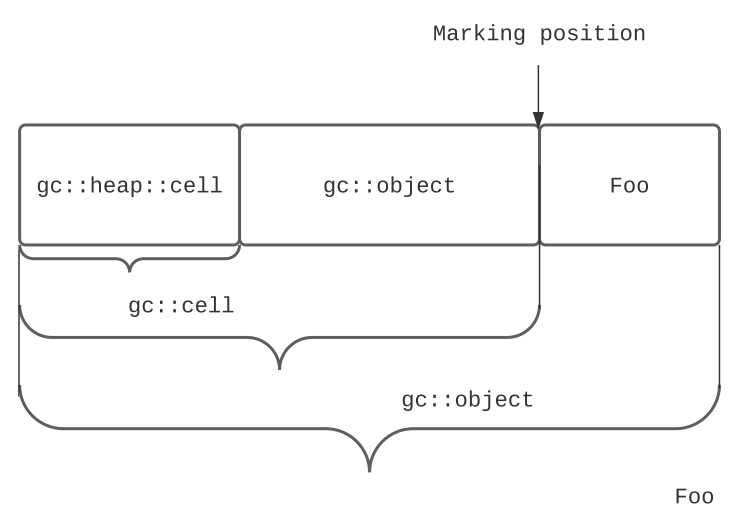
\includegraphics[scale=0.5]{./report_srcs/c_plus_plus_casting.png}
\end{center}
\caption{C++ Casting}
\label{fig:cppcasting}
\end{figure}

Because of this, and the fact that a class will inherit from the \texttt{gc::object} class, the marker is
positioned to start at \texttt{(((char*)this) + sizeof(gc::object))}. Because fields start at the beginning
of the user specified section of the object, this position can be assured to start at the initial field
(if there are any).
Due to the lack of reflection, the marker needs to work out when to stop marking by analysing the data at
the current marking position. This is achieved based on knowledge of how a field should be formatted.

Fields have to hold a reference to an object in the heap of a \texttt{nullptr} in order to be valid. Both formats
are easy to test:
\begin{itemize}
\item If the marker sees a \texttt{mullptr} at its current position it will accept this as a valid field
and move onto the next one.
\item If the marker sees a pointer address which is within the range of the heap it will mark the referenced
object and then move on to the next field.
\end{itemize}

Fields are ended with the \texttt{END\_GC\_FIELDS} macro. This macro actually adds a new member to the class of
type \texttt{void*} pointing to one position less than the allocated heap. The marker will look specifically 
for this pointer value when looping through the fields to mark. If it sees this value, it will know that it 
has marked the last field and can stop.

\subsubsection{Optimisation Attempts for Stopping Marking}
\subsection{Allocating}
AGC objects have an overidden \texttt{new} operator which calls the 
\texttt{gc::heap::heap\_struct::malloc} function to provide a suitable memory position 
in the heap.

\subsubsection{\texttt{gc::heap::heap\_struct::malloc}}
The \texttt{malloc} function uses the \texttt{attempt\_allocate} member function to find the
memory position. If this function returns a \texttt{nullptr}, this means that the function 
was unable to find a suitable memory position, and the system should attempt a garbage
collection before continuing.

\texttt{malloc} will attempt to allocate twice after two gc cycles, before giving up
and throwing a \texttt{bad\_alloc} exception. The reason for the double collection is 
to ensure that recently unreferenced objects have an opportunity to become freed when 
attempting to allocate as seen in figure \ref{fig:gcingobject}.
\begin{figure}
\begin{center}
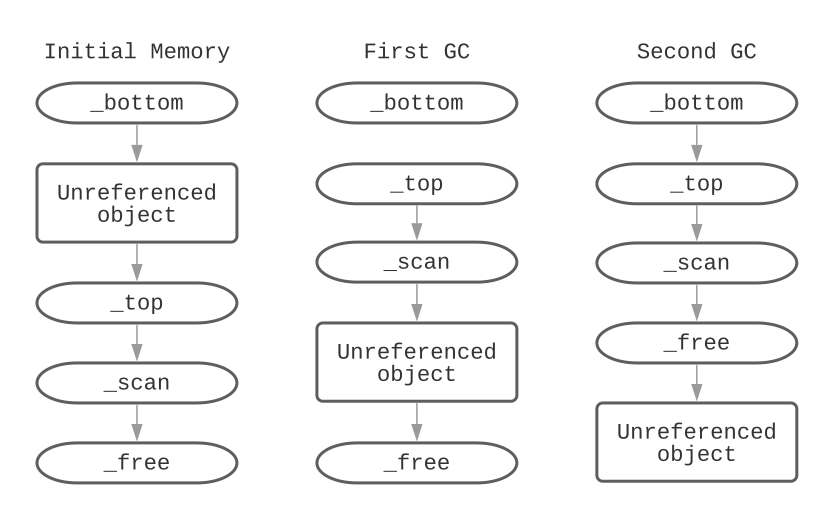
\includegraphics[scale=0.5]{./report_srcs/collecting_unreferenced_object.png}
\end{center}
\caption{Collecting an Unreferenced Object}
\label{fig:gcingobject}
\end{figure}

If the system is unable to allocate an object after two gc rounds, it is highly likely
that it is not possible to allocate the given object (This does however depend on the
number of alloed allocation loops, which will be discussed with regards to the
\texttt{attempt\_allocate} function).

Once \texttt{malloc} has been provided a suitable memory position it will re-adjust
teh position to take account of V-Table. In C++, objects that make use of virtual
functions start their memory allocation with a pointer to a V-Table to perform the
function lookup. AGC has two main kinds of structures that appear on the treadmill lists.
Initially the treadmill is set up with a single \texttt{gc::cell} in the free list
which is the same size as the given heap size. \texttt{gc::cell} does not have any virtual
functions, and as such does not begin its memory allocation with a V-Table reference.
\texttt{gc::object} however does start with a V-Table pointer (This is not necessarily
a requirement for it to function, but its currently kept like this to ensure that 
users can use virtual functions further down the inheritance tree).
The \texttt{gc::object} class also inherits from the \texttt{gc::cell} class which is the
reason for the need to reposition the memory position after allocation.
Links in the treadmill list always point to the \texttt{gc::heap::cell} object.
This is fine initially as the cell begins at the given pointer position.
\begin{figure}
\begin{center}
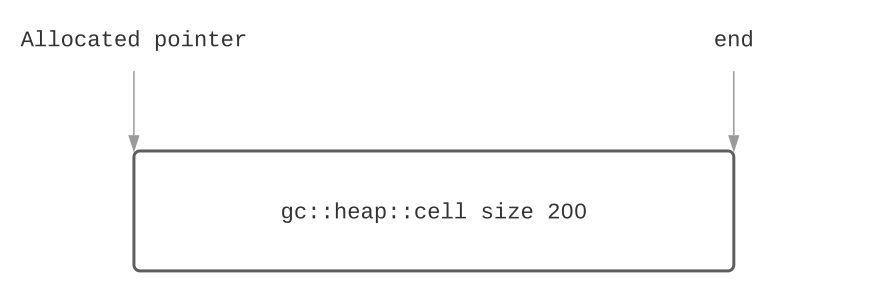
\includegraphics[scale=0.5]{./report_srcs/free_cell_allocation.png}
\end{center}
\caption{Positioning of pointer to free \texttt{gc::heap::cell}}
\label{fig:freecell}
\end{figure}

But this will not work if the cell is actually part of a now garbage collected object.
In this second case, the position of the cell object and the position of where that
cell actually is are different, due to the additional V-Table pointer
(Shown in figure \ref{fig:allocatedobject}).
\begin{figure}
\begin{center}
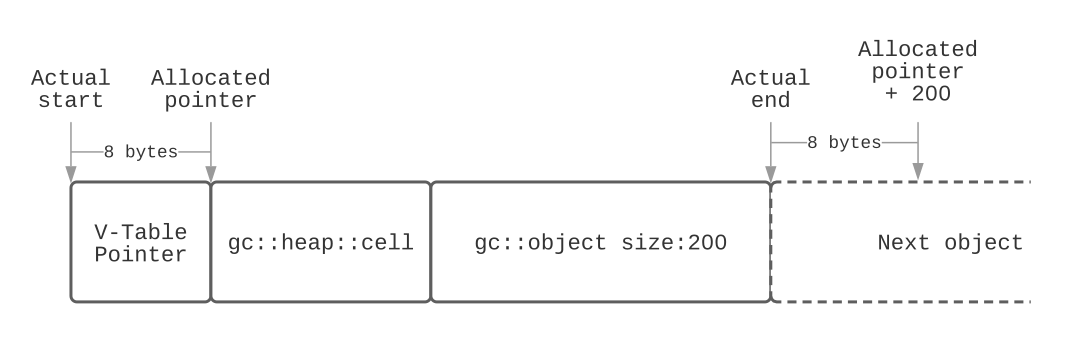
\includegraphics[scale=0.5]{./report_srcs/full_object_allocation.png}
\end{center}
\caption{Positioning of pointer to \texttt{gc::heap::cell} in a \texttt{gc::object}}
\label{fig:allocatedobject}
\end{figure}

\texttt{malloc} takes this information into account by calling the \texttt{gc::heap::cell::actual\_position} member function.
The contents of this function is set when a \texttt{gc::heap::cell} is constructed and gives the data as to whether the cell object
is at an offset or not. When a standard cell is created, this function will return the same as the \texttt{this} pointer, but if it
was constructed during the creation of a \texttt{gc::object} it will instead point to \texttt{this - sizeof(void*)}.
\texttt{malloc} must make this adjustment to ensure that any newly created object does not bleed data into the next heap position.
\texttt{malloc} will also add this cell to the initialization list. This is a blacklist that ensures that objects do not
get garbage collected before their initialisation has been finished. Without this safety, a sub-object \texttt{malloc}
could run out of memory and attempt to garbage collect its parent object's memory. Once the entire object has been fully constructed
(an event the system knows has taken place once the \texttt{field}/\texttt{static\_ptr} constructors havbe been reached), the objects
get removed from the initialisation list ready for possible garbage collection.

\subsubsection{\texttt{gc::heap::heap\_struct::attempt\_allocate}}
This function is responsible principally for finding free memory locations, and where necessary, merging contiguous cells
that exist in free memory, \texttt{attempt\_allocate} attempts to find allocation positions by comparing the new object's size
requirements to each cell in the free list, starting from the top of the list (\texttt{\_free} cell) and working down.
If a free cell is found which is large enough, it will break off an amount of memory which is equal to the size of the new cell.
If the new object size is the same as the free cell size, this is a very simple process. All that needs to
be done is to unlink the free cell from the free list and return the pointer. If however the free cell is larger, a cell
resize needs to take place by calling the \texttt{gc::heap::cell::resize} function.
Cell resizing is performed by moving the start of the free cell object forwards by an amount which is equal to the
size of the new object as seen in figure \ref{fig:initialresize}.
\begin{figure}
\begin{center}
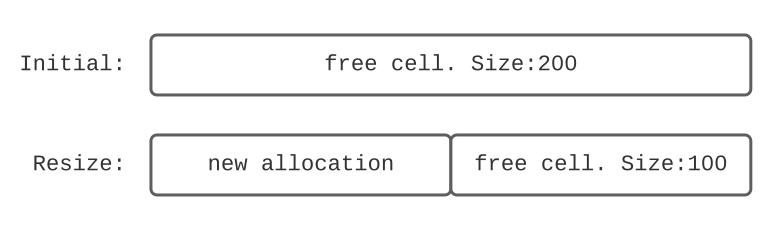
\includegraphics[scale=0.5]{./report_srcs/initial_to_resize.png}
\end{center}
\caption{Cell resize after new allocation}
\label{fig:initialresize}
\end{figure}

\texttt{gc::heap::cell} has a certain amount of data that needs to be stored, such as its size and positions in the treadmill
and location lists. Because of this, there is a minimum object size for a given cell. If it is found that the space left over in the free
cell is too small a cell  merge needs to be performed with one of its neighbours. \texttt{resize} will first attempt to 
merge the memory with its forward neighbour if this is not allocated memory. In this case, a new cell is created
at the position of the orphan memory, which will incorporate the orphan memory along with the forward cell
that it is being merged with.
\begin{figure}
\begin{center}
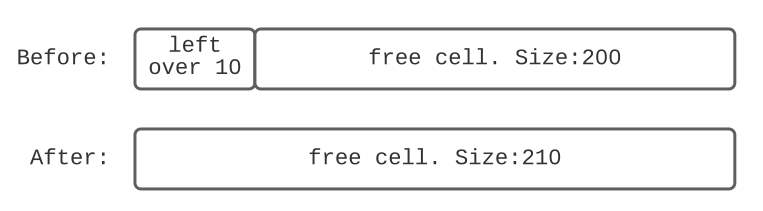
\includegraphics[scale=0.5]{./report_srcs/forward_merge.png}
\end{center}
\caption{Left over memory merging with forward free cell}
\label{fig:forwardmerge}
\end{figure}

If the forward object is allocated memory then it is not possible to merge without corruption of the object.
So instead, a merge with the back object (or more specifically our newly allocated object) is performed which will
simply act as padding on the end of the object allocation.

\begin{figure}
\begin{center}
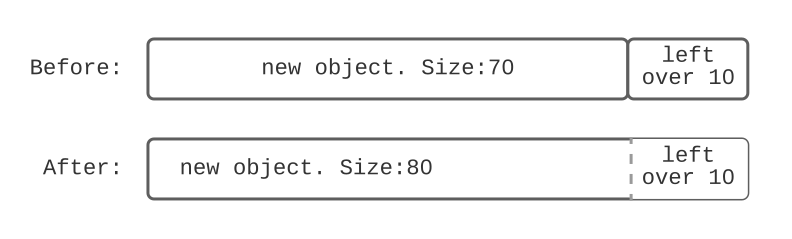
\includegraphics[scale=0.5]{./report_srcs/backward_merge.png}
\end{center}
\caption{Left over memory merging with backward, newly allocated object}
\end{figure}

If a free cell is not large enough to accommodate a new object size, \texttt{attempt\_allocate} will
attempt to merge the current free cell with its forward neighbour and try again. If it is unable to merge
with its forward neighbour it will move onto the next position in the free list and attempt the same
algorithm again. \texttt{attempt\_allocate} has a loop limit defined when the heap is first created as the 
\texttt{gc::heap::heap\_struct::\_max\_allocation\_attempts\_before\_gc} member.
Once the \texttt{attempt\_allocate} loop has been run this many times, the function will give up and 
return a \texttt{nullptr} in order to allow a garbage collection to take place to free up more memory.

\subsubsection{Detecting Free Cells in O(1) Time}
Detecting whether or not a cell is currently free or not is important in this system to ensure that
data does not get corrupted by cell merges. Because making this check needs to be performed on such a consistent
basis, it is alos important that the detection of free cells is a very fast process, in this case, an O(1) time process.

AGC's cell merge system uses the \texttt{gc::heap::cell::garunteed\_free} function to check to ensure
that a cell is definitely in the free list. It is important to note that not every free cell will return true
to this function depending on its current state. It only guarantees that no cell that returns true to this function
\textbf{has} to be free.

To do this, every \texttt{gc::heap::cell} has a byte member called \texttt{\_iteration}. This value corresponds to the 
byte member \texttt{gc::heap::heap\_struct::\_gc\_iteration}. \texttt{\_gc\_iteration} gets iterated every time a garbage collection
flip is performed and is used as a notification to all objects that their gc status has been changed.
\begin{enumerate}
\item \textbf{Use on Objects That are Still Allocated}

Objects need to keep track of what gc list they are currently in, in a fashion which can be accessed in
O(1) time. Objects do this by using the byte member \texttt{gc::object::\_mark} which can either be \texttt{W}, 
\texttt{G} or \texttt{B} for \textit{ecru}, \textit{grey} and \textit{black} lists respectively.
At different markers, the object will perform different actions when the \texttt{gc::cell::gc\_mark} member function is called.
\begin{itemize}
\item When in \textit{ecru}, the object moves to \textit{grey} and changes \texttt{\_mark} to \texttt{G}.
\item When in \textit{grey}, the object moves to \textit{black}, calls \texttt{gc::cell::gc\_mark} on all of its fields,
and changes \texttt{\_mark} to \texttt{B}.
\item When in \texttt{black}, no action is taken.
\end{itemize}
The \texttt{\_iteration} member becomes important once a gc flip occurs. In this case it will move objects in the \textit{black}
list to the \textit{ecru} list, but the objects still display an internal \texttt{\_mark} of \texttt{B} suggesting that it
thinks it is in a \textit{black} list, and should therefore do nothing when \texttt{gc\_mark} is called. Rather than slow down the gc flip
by manually setting each object back to \texttt{\_mark = 'W'}, instead the process is performed lazily by checking for inconsistencies
between \texttt{gc::heap::cell::\_iteration} \\
and \texttt{gc::heap::heap\_struct::\_gc\_iteration} during \texttt{gc\_mark} calls. If when \texttt{gc\_mark} is called the object sees
that its \texttt{\_iteration} value is behind \texttt{\_gc\_iteration}, it now knowz that a gc flip has occurred since and it needs to reset
to \texttt{\_mark = 'W'}.

\item \textbf{\texttt{\_iteration} in Free Cell Merges}

This same \texttt{\_iteration} member is also used in determining if a cell can be merged with. Because cells that are currently 
allocated are required to update their \texttt{\_iteration} member every gc cycle to keep in sink with the global
\texttt{\_gc\_iteration}, this fact can then be exploited in order to tell which cells are not being updated. It can
be garunteed that any cell which has an \texttt{\_iteration} value that is not equal to \texttt{\_gc\_iteration}
of \texttt{(\_gc\_iteration - 1)} is actually a free cell.
\begin{itemize}
\item Where \texttt{\_iteration = \_gc\_iteration}, the cell must have either recently updated their member, or have
been allocated in the current iteration and are therefore not free
\item Cells that have \texttt{\_iteration = (\_gc\_iteration - 1)} must either not yet have had the change to update their masrk
yet, or have just been freed in the previous cucle.
\end{itemize}

If any other \texttt{\_iteration} value is found, then we must conclude that the cell is out of date and garunteed to be free.
Because \texttt{\_iteration = (\_gc\_iteration - 1)} can be true on an allocated cell, this means that it only becomes possible
to merge with a free cell once two garbage collections have passed since it was first placed in the free list.
\end{enumerate}

\subsection{Object Survival and Being Unreferenced}
The standard approach for memory management in C++ is to perform reference counting, that is, to count the number of 
references that are pointing to a given object, and then once no references are left, delete the object. AutoGarbage uses
mark and sweep which will instead, as the program is being executed, gradual;ly mark out and reveal the memory cells which are still
being referenced.
The underlying effect of this method of memory management is that objects tend to stay allocated a little longer than they 
are atually required to be. This means that the amount of memory used by a program at any time is going to be slightly greater
than what is actually require, simply because a gc cycle has yet to occur, or an objects gets sent to the grey/black list 
just before it gets dereferenced.

This expanded object lifetime can mean that on occasion, a greater computational overhead is associated with
mark and sweep as it can take a couple of cycles for an unreferenced object to finally be freed. Specifically in the AutoGarbage
system, it may even take yet another cycle to become a genuinely useful allocatable object, due to the approach taken to ensuring
that it is safe to merge with free cells.

\newpage
\appendix
\section{Other Approaches Explored for Stopping Marking}
\label{app:exploredmarkingapproaches}
A few other approaches were explored to perform the task of stopping the marker as it explores an object prior to the magic
pointer algorithm that is currently being used within the AutoGarbage program with the goal of reducing the overall memory overhead
of objects. 

The magic pointer technique (figure \ref{fig:mark:magicpointer}) requires an 8 byte overhead on 64 bit systems.
This compares to a field flag technique (figure \ref{fig:mark:fieldmemberflag}) which would
have added a byte to the top of the field class which could have a different value to a \texttt{END\_GC\_FIELDS} added member byte 
at the end of the field list. This approach is better so long as a class has fewer than 7 fields (each field has an extra byte 
along with the \texttt{END\_GC\_FIELD} byte makes the 8 bytes taken by the magic pointer technique).
A slightly different approach that could be taken is to reserve the top bit of the fields pointer to use in the marking system (figure \ref{fig:mark:onpointerflag})
(set to 0 on fields). This approach would allow for an overhead of only a single byte at the expense of reducing the addressable 
heap memory from 64bits to 63.

Unfortunately due to the prominence of little endian formatted computers, applying the current system while only observing the most
significant byte cannot be used as an optimisation. On big endian machines, a magic number could be used checking only the most
significant byte and omitting the rest of the pointer bringing the overhead back to just a single byte without reducing
addressable space.

The likely best approach that may be worth moving to in future is the single bit flag within the pointer. This is because although
it does reduce addressable space, it only reduces 
it from a possible $\sim$18 exabytes to $\sim$9 exabytes\textsuperscript{[\ref{app:addessablespace}]},
memory spaces that are well beyond even the largest super computers\textsuperscript{\cite{bib:summitsupercomputer}}


\begin{figure}
\begin{center}
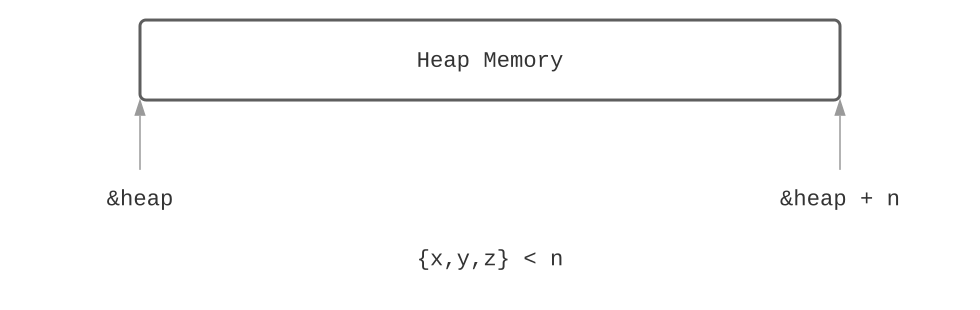
\includegraphics[scale=0.5]{./report_srcs/heap_memory_only.png}
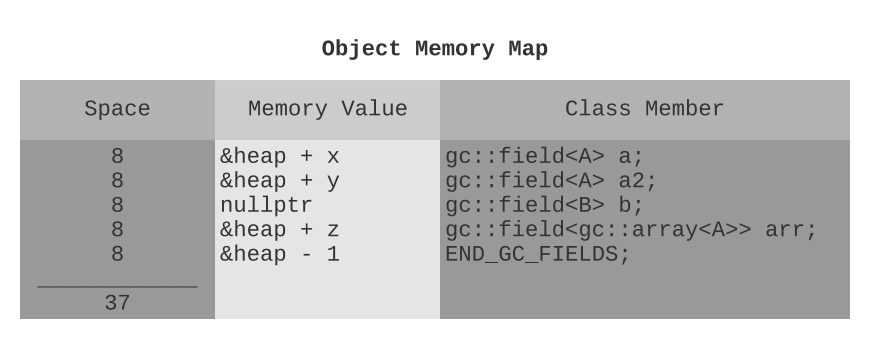
\includegraphics[scale=0.5]{./report_srcs/magic_pointer_technique.png}
\caption{Magic Pointer Technique}
\label{fig:mark:magicpointer}
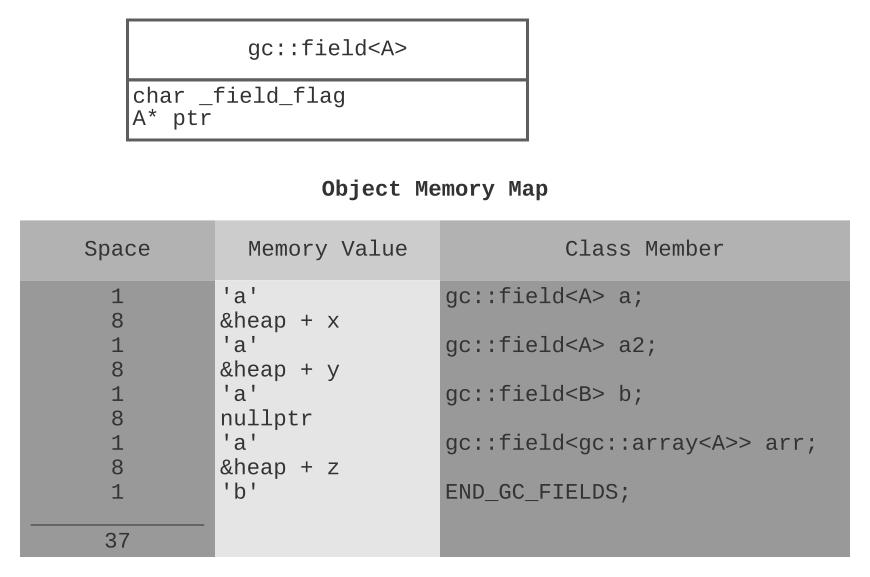
\includegraphics[scale=0.5]{./report_srcs/field_member_flag_technique.png}
\caption{Field Member Flag Technique}
\label{fig:mark:fieldmemberflag}
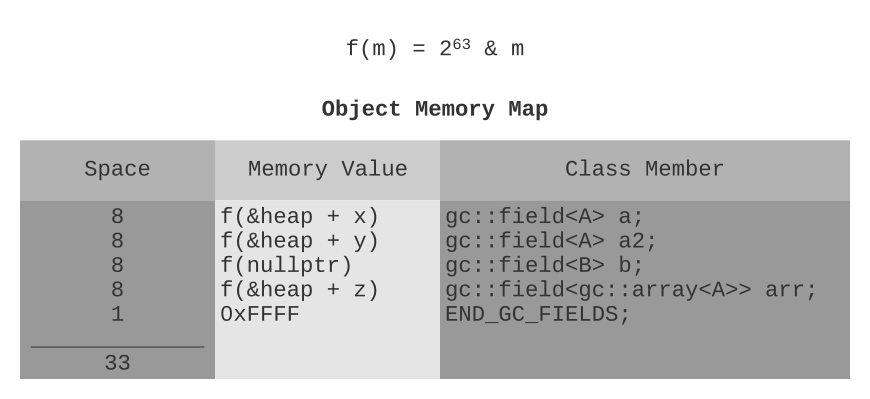
\includegraphics[scale=0.5]{./report_srcs/on_pointer_bit_flag_technique.png}
\caption{On Pointer Bit Flag Technique}
\label{fig:mark:onpointerflag}
\end{center}
\end{figure}

\subsection{Addressable Space}
\label{app:addessablespace}
Addresses in C++ direct to individual bytes. The maximum possible unsigned 64 bit number is
18,446,744,073,709,551,614. This therefore is approximately 18 exabytes which is addressable. One bit
used as a separate flag, reduces to $2^{63}$ addresses hence 9 exabytes addressable.

\section{Separate Thread Marking for Multi-Threaded Environments}
\label{app:multithreadedmarking}
The current AutoGarbage system performs marking of memory when the program makes accesses to objects
or when it has run out of memory during an allocation. Another approach that can be taken is to 
queue up objects to be marked as they get accessed and use a different thread to take objects off of the querue
and mark them. This approach decouples the programmers threads from the marking process, ensuring that multiple threads
can access the object at the same time without having to worry about performing the correct marking
procedure in accordance with the object's current state.

\newpage
\begin{thebibliography}{9}
\bibitem{bib:summitsupercomputer}
2018 Summit Super Computer at Oak Ridge National Laboratory

2,801,664 GB of volatile memory (4,608 nodes of 512 GB DDR4 + 96 GB HBM2)
\texttt{https://www.olcf.ornl.gov/summit/}
\bibitem{bib:treadmillgc}
Baker, Henry. (1995). The Treadmill: Real-Time Garbage Collection Without Motion Sickness. 

%Concurrent mark and sweep for java, probably worth mentioning
%https://docs.oracle.com/javase/8/docs/technotes/guides/vm/gctuning/cms.html

%If intending on looking at future possible generational systems also look to java docs
\end{thebibliography}
\end{document}